% Paper draft for FPGA 2013
\pdfminorversion=5
\documentclass[conference]{IEEEtran}
\usepackage[binary-units]{siunitx}
\sisetup{detect-weight=true, detect-family=true}
\usepackage{enumitem}
\usepackage{graphicx}
\usepackage{multirow}
\usepackage[caption=false,font=footnotesize]{subfig}
\usepackage{dblfloatfix}
\usepackage{xspace}
\usepackage{url}
%\usepackage[square, comma, sort&compress, numbers]{natbib}
\usepackage{algorithm}
\usepackage{algorithmic}
\usepackage[algo2e]{algorithm2e}
\usepackage{amsmath}
\usepackage{bm}
\usepackage[table]{xcolor}
\usepackage{tablefootnote}

% \usepackage{draftwatermark}%
% \SetWatermarkFontSize{20cm}%
% \SetWatermarkScale{2}%
% \SetWatermarkText{DRAFT Do not distribute}%

\setlength{\parskip}{0pt}
\renewcommand{\topfraction}{1}
\renewcommand{\textfraction}{0.15}
\renewcommand{\dbltopfraction}{1}

\renewcommand\floatpagefraction{.9}
\renewcommand\topfraction{.9}
\renewcommand\bottomfraction{.9}
\renewcommand\dbltopfraction{.9}
\renewcommand\textfraction{.1}   
\setcounter{totalnumber}{4}
\setcounter{topnumber}{8}
\setcounter{bottomnumber}{4}
\setcounter{dbltopnumber}{4}

\newcommand*{\Scale}[2][4]{\scalebox{#1}{$#2$}}
\newcommand{\eqnref}[1]{Equation~\ref{#1}}
%\newcommand{\eqnref}[1]{(\ref{#1})}
\newcommand{\figref}[1]{Figure~\ref{#1}}
\newcommand{\algref}[1]{Algorithm~\ref{#1}}
\newcommand{\secref}[1]{Section~\ref{#1}}
\newcommand{\tabref}[1]{Table~\ref{#1}}
\newcommand{\code}[1]{\texttt{#1}}
\newcommand{\tabincell}[2]{\begin{tabular}{@{}#1@{}}#2\end{tabular}}
\renewcommand{\algorithmcfname}{ALGORITHM}
\SetAlFnt{\small}
\SetAlCapFnt{\small}
\SetAlCapNameFnt{\small}
\SetAlCapHSkip{0pt}
\IncMargin{-\parindent}

\graphicspath{{./figures/}}

\begin{document}
\bstctlcite{IEEEexample:BSTcontrol}
\title{AccSim: A Flexible Memory Simulator for Hardware Accelerator Simulation}

\author{\IEEEauthorblockN{xxx, xxx and xxx}
\IEEEauthorblockA{School of Computing\\
National University of Singapore\\
Email: \{xxx\}@xxx}
}
\maketitle

\begin{abstract}
With the advancement of the FPGA techniques and the increase of successful demonstrations 
of using FPGAs in data center, more and more cloud computing vendors start to integrate 
FPGAs as computing resources in the cloud. In order to make best use of the computing resources 
in the cloud, the computing resources are usually virtualized such that they can be shared by different 
computing tasks from either a single user or multiple users. Nevertheless, unlike the 
conventional computing resources such as CPUs and GPUs, FPGAs are difficult to be virtualized 
and shared at runtime for two reasons. On the one hand, the same FPGA design requires lengthy implementation 
targeting different types of FPGA devices and thus the same task can't be migrated to 
a different type of FPGA device. On the other hand, 
CGRA overlay which is an intermedaite layer built on top of FPGAs can be shared by 
different applications and also allows efficient runtime context switch. Thus we explores 
CGRA overlay for the FPGA resource virtualization. 



The design productivity of FPGA development which remains magnitudes lower compared to typical software development severely hinders the widespread adoption of FPGAs. Particularly, the lengthy low-level FPGA implementation process including synthesis, placing and routing dramatically limits the number of compile-debug-edit cycles per day and lowers the FPGA design productivity. To address this design productivity problem, we have developed a rapid FPGA loop accelerator generation framework called QuickDough. Instead of trying to reduce the implementation time, it reuses a pre-built accelerator library to avoid the lengthy implementation process during design iterations. By utilizing a soft coarse-grained reconfigurable array (SCGRA) overlay built on top of off-the-shelf FPGAs as the backbone of the accelerators in the library, it compiles a high-level loop to the FPGA through a rapid operation scheduling first and then generates the FPGA accelerator bitstream through a rapid integration of the scheduling result and a pre-built accelerator bitstream selected from the library. According to the experiments, QuickDough is able to produce accelerators in the order of seconds while achieving up to 9X performance speedup over the execution of the same software running on a hard ARM processor.  

\end{abstract}
 
% A category with the (minimum) three required fields
%\category{H.4}{Information Systems Applications}{Miscellaneous}
% A category including the fourth, optional field follows...
%\category{D.2.3}{Hardware Engineering}{Metrics}[complexity measures, performance measures]
%\terms{Theory}
%\keywords{High Level Synthesis, Soft Coarse Grain Reconfigurable Array, Design Productivity, High Frequency FPGA Design}

\section{Introduction}
Improving general-purpose processing system is getting extremely 
difficult. More and more computer architects believe that the major 
improvements in cost-energy-performance will come from domain-specific 
hardware accelerators. Recent years have already seen a number of successful 
demonstrations utilizing domain specific hardware accelerators for critical 
domains of applications such as deep neural network \cite{Jouppi2017tpu, Li2017survey} 
database operations \cite{Wu2014q100} and graph processing \cite{Jun2016graphicionado, Ozdal2016energy}. 
In order to explore the hardware accelerator design, a hardware accelerator simulator 
is usually required. Indeed there are already many exisitng tools \cite{systemc, chisel} and 
models \cite{dramsim2, ramulator} that can be used to help with the hardware accelerator 
design, it is non-trivial to develop a hardware accelerator on top of these work. For instance, there 
is a lack of general public cycle-accurate memory models available in \cite{systemc, chisel} while 
\cite{dramsim2, ramulator} expose only primitive memory access interface and need to be further 
wrapped for an accelerator simulator. And a general accelerator simulator 
framework is highly desired for the hardware accelerator simulator development.

Despite the difference of the accelerator simulators, we argue that a general 
accelerator simulator design framework should have three common yet important 
features. First of all, it should provide memory models of various memory 
architectures. Basically memory is usually critical to the hardware accelerator 
and greatly affects the accelerator design. At the same time, memory techniques evolve rapidly 
over the years and novel memory architectures with distinct features emerge. In order to explore 
hardware accelerator design, various memory architectures needs to be evaluated. 
Secondly, it should provide abstract user-frinedly memory interfaces. Hardware accelerators 
usually have complex memory access patterns such as stream access, burst access as well as random access. 
Thus higher abstract memory access interface instead of primitive memory access interface should be provided. 
Thirdly, it should provide trade-off between simulation speed and precision. Hardware accelerators 
may have distinct simulation speed and precision requirements while exploring the hardware accelerator. 
For instance, some of the applications such as graph accelerators may process on a big data set. 
Low-level accurate memory model may result in extremely long simulation. Thus a simplified memory model 
should be used to obtain the general performance of the accelerators. For applications that are sensitive 
to the memory access latency, more accurate memory models are preferred.

There is still a lack of general accelerator simulator framework that fullfills 
all the three features mentioned above. To that end, we proposed a flexible hardware accelerator 
simulation framework to be reused for general hardware accelerator simulator development. Basically, it 
integrates ramulator supporting various memory architectures as the underlying memory model and thus allows 
hardware accelerator exploration over a broad range of memory architectures. In addition, abstract memory 
interfaces as well as memory content management are provided to faciliate the accelerator accessing 
the memory model. Finally, it also provides a mix of cycle-accurate memory model and simiplified 
analytical memory model obtained though sampling to compromise on simulation speed and accuracy.

The rest of the paper is organized as follows. Section 2 is the realted work, Section 3 presents 
the proposed accelerator simulation framework. Section 4 provides the experimental results 
and Section 5 concludes this paper.






\section{Related Work} \label{sec:relatedwork}
Despite of the performance and power advantages, the design 
productivity of developing FPGA applications remains low 
due to the lengthy compilation and complex application-specific 
customization. And it has become the major obstacle 
that hinders the wide adoption of FPGAs as commodity computing devices. 
The community from both the industry and academia have developed 
many different methods from diverse angles to tackle the problem. 
These methods can be roughly classified into three categories. 
The first category mainly focuses on improving the low-level 
implementation tools. A number of approaches such as making 
quality/runtime trade-offs \cite{mulpuri2001runtime}, parallel 
compilation \cite{moctar2014parallel, goeders2011deterministic, altera-pc, 
xilinx-pc} and using hard-macro techniques \cite{lavin2013improving, 
korf2011automatic} have been explored from this angle. The second 
category mainly centers the HLS design flow while the third one 
primarily relies on the overlay concept. They later two categories 
will be detailed in the following sections.

\subsection{High-Level Synthesis} 
With many years of continuous endeavor, a number of tools have emerged as 
mature solutions for HLS \cite{VivadoHLS, Legup, zhang2008autopilot}. They typically 
allow designers to express hardware designs using high-level  
description languages such as C, C++ etc. and also enable evaluation of different 
design choices using pragmas or directives. Indeed, they significantly improve 
the design productivity compared to the conventional hardware design flow using 
hardware description languages. However, when considering the overall design 
productivity of developing hybrid software-gateware applications, HLS is 
only addressing part of the problem, as the lengthy low-level compilation 
including synthesis, mapping, placing and routing remains a bottleneck for 
an application designer \cite{ROB2014, capalija2014tile}.

Customizing the generated hardware specifically to an user 
application is also time-consuming for designers and thus critical to the design 
productivity. A number of algorithms such as generic algorithms 
relied on local-search techniques \cite{schafer2009adaptive, 
sengupta1997genetic}, learning-based methods \cite{onlinecustomization, 
carrion2012machine}, divide and conquer algorithm \cite{DCcustomization} 
and a calibration free algorithm \cite{RCcustomization} etc. have been developed 
to perform the DSE on top of HLS tools. The algorithms can efficiently help automate the 
customization or DSE process. However, the algorithms must rely on HLS tools 
to estimate the implementation information such as implementation frequency, 
overhead or power for the corresponding customization. While the hardware generated 
can be irregular and may vary dramatically, thus the accuracy of the estimation 
especially on implementation frequency and power can be rather limited, which may
fail to optimize an HW/SW co-design problem.  

\subsection{Overlay Architectures}
Overlay architecture which is a virtual intermediate architecture overlaid on 
top of off-the-shelf FPGA is increasingly applied as a way to address the 
productivity challenge. 

Various overlays with diverse configuration granularities and flexibility 
ranging from virtual FPGAs \cite{Grant2011Malibu, ZUMA2012}, 
array-of-FUs \cite{mesh-FUs,ferreira2011fpga}, soft 
CGRA \cite{kissler2006dynamically, scgra-orig}, soft GPU \cite{Guppy2012GPU-Like}, 
vector processors\cite{Yiannacouras2009FPS, MXP2013} to 
configurable processors or multi-core processors \cite{unnikrishnan2009application, 
MARC2010, Yiannacouras2007Exploration, Capalija2009coarse-grain, OCTAVO2012, iDEA2012} 
have been developed over the years. SCGRA overlay provides unique 
advantages on compromising hardware implementation 
and performance for compute intensive nested loops as demonstrated 
by numerous ASIC CGRAs \cite{tessier2001reconfigurable, compton2002reconfigurable}.
Most importantly, it allows both rapid compilation by taking advantage of 
the overlays' tiling structure \cite{ROB2014} and efficient bitstream 
reuse within the design iterations of an application \cite{scgra-orig}, 
thus it is particularly promising for high productivity nested loop acceleration.

Despite of the promising potential, a complete automatic customization 
framework that enables application-specific optimization is still highly 
anticipated for the sake of design productivity and performance. 
The authors in \cite{colinheart} developed an SCGRA topology customization method 
using genetic algorithm and showed the potential benefits of the SCGRA 
overlay customization. However, the rest system design parameters such as 
on chip buffer size, loop unrolling factor etc. are not covered. 

Indeed, SCGRA overlays have many similarities in terms of array structure 
and scheduling algorithm with ASIC CGRAs. Nevertheless, ASIC CGRAs emphasize 
more on configuration capability and limited customization is allowed due 
to the overhead constraints \cite{zhou2014application, miniskar2014retargetable} 
while SCGRA overlays allow more intensive architectural customization 
because of the FPGA's inherent programmability. Moreover, hardware resources such as 
DSP blocks and RAM blocks available on FPGAs are discrete, which results in different 
design constraints for SCGRA overlay customization as well. 

By utilizing the SCGRA overlay as the backbone of the FPGA accelerator, 
a complete nested loop acceleration framework 
targeting CPU-FPGA system is developed. It supports intensive application-specific
customization including the overlay architectural customization, 
the compilation customization and communication interface customization 
for various design goals. When the customized design parameters are determined, 
corresponding hardware accelerator and software can be compiled to the target 
CPU-FPGA system rapidly eventually providing a push-button solution for a nested loop 
acceleration. 



\section{Automatic Nested Loop Acceleration Framework} \label{sec:acc-framework}
By using a regular SCGRA overlay built on top of the physical FPGA devices, 
we have developed an automatic nested loop acceleration framework targeting 
a hybrid CPU-FPGA system. The goal of the framework is to provide a 
high-productivity nested loop acceleration solution accessible to high-level 
application developers as well as a rapid application-specific 
customization process to achieve better performance-energy trade-off of 
the resulting accelerators. 

\figref{fig:framework} shows the nested loop acceleration framework. Given 
a specified compute intensive loop kernel and high-level design 
goals as well as constraints, the framework automatically 
tunes the design parameters including the SCGRA overlay 
configuration, compilation options and on chip 
communication specifically to the loop kernel through the SCGRA customization 
process. After the customization, corresponding SCGRA overlay based 
FPGA accelerator is generated and implemented through the SCGRA compilation process. 
Meanwhile, the drivers that are needed to utilize the resulting FPGA accelerator 
are generated according to the SCGRA customization. Then the high level application 
is updated and compiled to general purposed processor (GPP) through a 
conventional software compilation process. The application binary code generated in 
combination with the FPGA accelerator bitstream forms the final application 
that will be executed on the hybrid CPU-FPGA system during run time.

\begin{figure}[tb]
\center{\includegraphics[width=0.75\linewidth]{framework}}
\caption{Automatic nested loop acceleration framework}
\label{fig:framework}
\end{figure} 

SCGRA customization process is the focus of this work where optimal 
design choices are decided. Since it involves exploration in a vast 
design space, it is critical to the design productivity of the whole 
framework. In addition, it also determines the configurations of 
the resulting accelerators and thus affects the performance-energy 
trade-off of the final design. In this work, a dedicated customization 
method is proposed to meet both the requirements of the design productivity and 
performance-energy trade-off and it will be further illustrated in the following 
sections.

SCGRA compilation is responsible for mapping the high-level loop 
kernel to the physical FPGA bitstream through a specified SCGRA 
overlay. \figref{fig:horizontal-compilation} presents an overview of the 
compilation process and it includes two compilation flows for two typical
development scenarios i.e. initial compilation and iterated compilation. 
In the first scenario when the specified SCGRA overlay is initially 
implemented on the target physical FPGA device, a standard implementation 
from HDL model may be time-consuming. Fortunately, a hardware-macro compilation 
technique \cite{ROB2014} developed for the regular tiling architectures may 
significantly decrease the implementation time. In the second scenario when 
the specified SCGRA overlay has already been implemented, the bitstream can 
be reused as demonstrated in \cite{scgra} and the compilation can be reduced to seconds.

\begin{figure}[tb]
\center{\includegraphics[width=0.8\linewidth]{horizontal-compilation}}
\caption{High-productivity SCGRA overlay compilation, The whole diagram represents the initial
compilation and it includes both the iterated compilation and the initial implementation.}
\label{fig:horizontal-compilation}
\end{figure}



\section{SCGRA Overlay Based FPGA Accelerator Customization} \label{sec:customization-framework}
Application-specific customization provides unique opportunity to improve 
the energy and performance of the resulting accelerators. However, 
taking the system as a black box and exhaustively searching all the 
possible configurations can be inefficient and slow. In this work, by taking advantage 
of the regularity of the SCGRA overlay based FPGA accelerator, we 
can reduce the complex customization problem to a much simpler sub design space exploration (DSE)
together with a simplified search problem and optimized application-specific 
nested loop accelerator can be produced efficiently.

\subsection{Customization problem formulation}
In this section, we will formalize the customization problem of the nested loop acceleration on an
SCGRA overlay based FPGA accelerator. Various design constraints including energy consumption and
hardware resource overhead can be used while hardware overhead is taken as an example here.

\begin{table}[tb]
    \begin{threeparttable}
\scriptsize
\centering
\caption{Design Parameters of Nested Loop Acceleration\label{tab:parameter-list}}{
\begin{tabular}{l|l|l}
\hline
\multicolumn{2}{l|}{Design Parameters} & Denotation \\ \hline
\multirow{2}{*}{\tabincell{l}{Nested Loop \\ Compilation}} & Loop Unrolling Factor & $\bm{u}=(u_0,u_1, ...)$  \\ \cline{2-3} 
                                                           & Grouping Factor & $\bm{g}=(g_0, g_1, ...)$ \\ \hline
\multirow{11}{*}{\tabincell{l}{Overlay \\ Configuration}}  & SCGRA Topology  & Null, 2D Torus \\ \cline{2-3} 
                                                          & SCGRA Size  & $r\times c$ \\ \cline{2-3}
                                                          & Instruction Mem & $imD \times imW$ \\ \cline{2-3}
                                                          & Data Mem & $dmD \times dmW$ \\ \cline{2-3}
                                                          & Input Buffer & $ibD \times ibW$ \\ \cline{2-3}
                                                          & Output Buffer & $obD \times obW$ \\ \cline{2-3}
                                                          & Input Address Buffer & $iabD \times iabW$ \\ \cline{2-3}
                                                          & Output Address Buffer & $oabD \times oabW$ \\ \cline{2-3}
                                                          & Operation Set & Null, fixed \\ \cline{2-3}
                                                          & Implementation Frequency & $f$, fixed \\ \hline
                                                          & Pipeline Depth & Null, fixed \\ \hline
\end{tabular}
\begin{tablenotes}
    \small
\item Null means there is no denotation for that parameter.
\end{tablenotes}
}
\end{threeparttable}
\end{table}

Suppose $\bm{\Psi}$ represents the overall nested loop acceleration design 
space. $\bm{C} \in \bm{\Psi}$ represents a possible configuration in 
the design space and it includes a number of design parameters as  
listed in \tabref{tab:parameter-list}. Assume that the loop to be accelerated 
has $n$ nested levels and loop count can be denoted as $l=(l_1, l_2, ..., l_n)$.
$R=(R_1, R_2, R_3, R_4)$ stands for the FPGA resource (i.e. BRAM, DSP, LUT and FF) 
that are available on a target FPGA and $Overhead(\bm{C}, i)$ denotes the 
four different types of FPGA resource overhead. $In(\bm{g})$ and $Out(\bm{g})$ 
stand for the amount of input and output of a group. Similarly, $In(\bm{u})$ 
and $Out(\bm{u})$ stand for the amount of input and output of a DFG. 
$DFGCompuTime(\bm{C})$ represents the number of cycles needed to 
complete the DFG computation. $\alpha_i$ and $\beta_i$ are constant 
coefficients depending on target platform where $i=(1,2,...)$. With these denotations, 
the customization problem targeting minimum energy consumption can be formulated 
as follows:

Minimize 
\begin{equation} \label{eq:runtime}
    \scriptsize
    RunTime(\bm{C})=CompuTime(\bm{C})+CommuTime(\bm{C})
\end{equation}
subject to
\begin{equation} \label{eq:constraints}
    \scriptsize
    \begin{split}
        &Overhead(\bm{C}, i) \leq R_i, i=1,2,3,4 \\
        &In(g) \leq ibD \\
        &Out(g) \leq obD \\
        &DFGCompuTime(\bm{C}) \leq imD \\
        &\displaystyle \prod_{i=1}^{n} \frac{g_i}{u_i} \times In(u) \leq iabD \\
        &\displaystyle \prod_{i=1}^{n} \frac{g_i}{u_i} \times Out(u) \leq oabD
    \end{split}
\end{equation}

$RunTime(\bm{C})$ represents the number of cycles needed to compute the loop on 
the CPU-FPGA system. It consists of both the time consumed for computing on FPGA and 
communication between FPGA and host CPU, and it can be calculated using \eqnref{eq:runtime}.

Since the unrolled part of the loop will be translated to 
DFG and then scheduled to the SCGRA overlay. Thus the DFG computation time 
is essentially a function of $\mathbf{u}$, $r$ and $c$, and it can also be 
denoted by $DFGCompuTime(\mathbf{u},r,c)$.
The nested loop is computed by repeating the same DFG execution, and the 
nested loop computation can be calculated using \eqnref{eq:loopexetime}.
\begin{equation} \label{eq:loopexetime}
    \scriptsize
    CompuTime(\bm{C})=\displaystyle \prod_{i=1}^{n} \frac{l_i}{u_i} \times DFGCompuTime(\mathbf{u},r,c)
\end{equation}

DMA is typically used for the bulk data transmission. Communication cost per 
data can be modeled with a piecewise linear function and thus DMA latency can be 
calculated using $DMA(x)$ where $x$ represents the amount of DMA transmission. The communication
time of the whole nested loop can be calculated by \eqnref{eq:commu}.
\begin{equation} \label{eq:commu}
    \scriptsize
    CommuTime(\bm{C})=\displaystyle \prod_{i=1}^{n} \frac{l_i}{g_i} \times 
    (DMA(In(\mathbf{g}))+DMA(Out(\mathbf{g})))
\end{equation}

Hardware overhead on FPGA mainly includes DSP, LUT, FF and 
BRAM (block RAM). LUT, FF and DSP overhead can be roughly estimated 
with a linear function of SCGRA size and can be calculated using \eqnref{eq:dsplutff}. 
BRAM overhead which is usually the overhead bottleneck for SCGRA overlay based 
FPGA accelerator design can be calculated by \eqnref{eq:bramoverhead}.
\begin{equation} \label{eq:dsplutff}
    \scriptsize
    Overhead(\bm{C}, i)=\alpha_i \times r \times c + \beta_i, (i=2,3,4)
\end{equation}
\begin{equation} \label{eq:bramoverhead}
    \scriptsize
    \begin{split}
        Overhead(\bm{C}, 1)=&r \times c \times (imD \times imW + dmD \times dmW) + \\
                               &(ibD \times ibW + obD \times obW) + \\
                               &(iabD \times iabW + oabD \times oabW) 
    \end{split}
\end{equation}
\subsection{Customization framework}
\figref{fig:customization-framework} illustrates the overview of the 
customization framework. It can be roughly divided into two 
parts. In the first part, a sub DSE targeting loop execution time 
is performed and the feasible design space can be obtained. Since loop 
execution time is determined by the operation scheduling 
which simply depends on the loop unrolling factor and SCGRA size, the 
sub DSE is much simpler compared to the overall system DSE which includes more than 10 design
parameters. In the second part, each configuration 
in the feasible design space will be evaluated. Instead of using simulation 
based methods, analytical models are employed to estimate the accelerator 
metrics such as performance and overhead. These analytical models are accurate because of the
regularity of the SCGRA overlay. Even though the feasible design space is still large, it is fast to evaluate 
all the configurations in it. After the evaluation process, customization for best performance
becomes trivial and the customized design parameters can be obtained immediately.

\begin{figure}[t]
\center{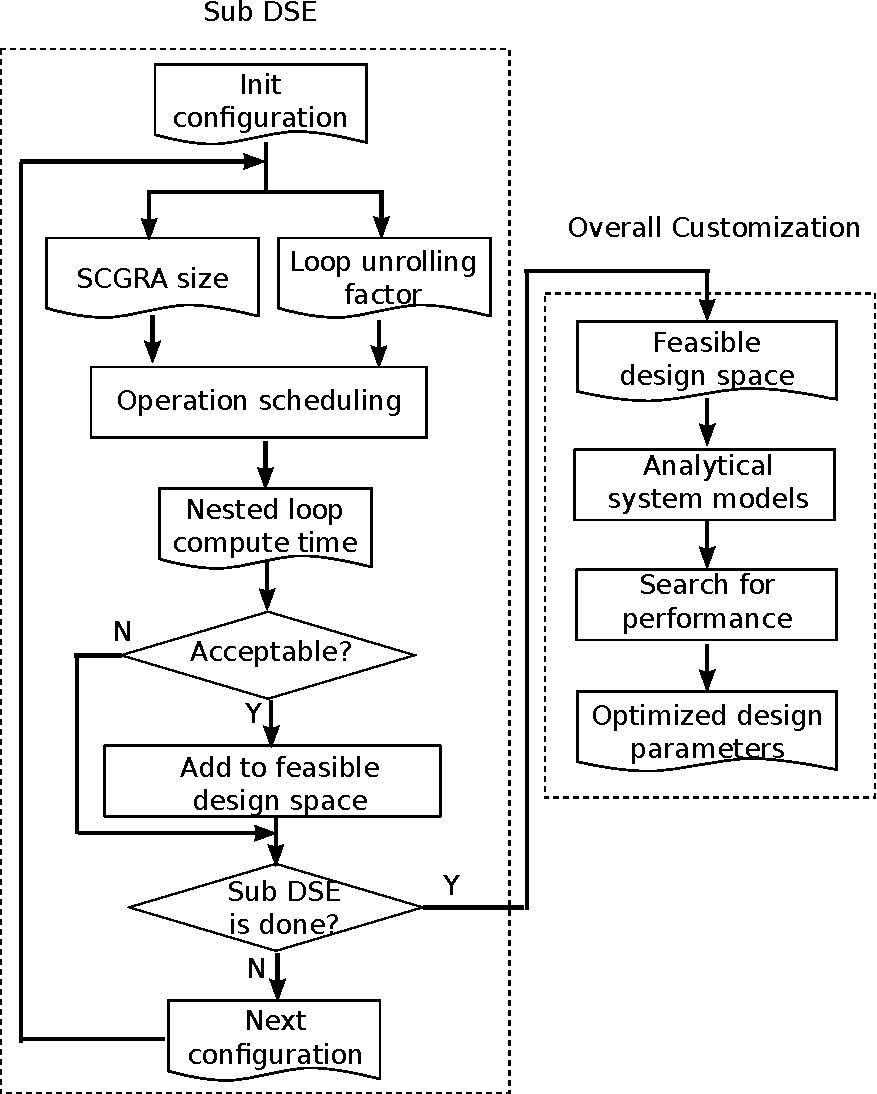
\includegraphics[width=0.8\linewidth]{customization-framework}}
\caption{System customization framework.}
\label{fig:customization-framework}
\end{figure}

Suppose $\Phi$ denotes the feasible design space. $\epsilon$ indicates the
percentage of the performance benefit obtained by the increase 
of loop unrolling or SCGRA size. It is a user defined 
threshold and must be small enough to prune the configurations that are 
inappropriate. The configurations in $\Phi$ must satisfy \eqnref{eq:cond1} 
and \eqnref{eq:cond2}. 
\begin{equation} \label{eq:cond1}
    \scriptsize
    \begin{split}
        &\forall \bm{C}=(...,\bm{u},r,c,...)\in \Phi, \bm{C'}=(...,\bm{u'},r',c',...) \in \Phi,\\ 
        & (r+1==r' \text{ and } c==c') \text{ or } (r==r' \text{ and } c+1==c'): \\ 
        &\frac{CompuTime(\bm{C})-CompuTime(\bm{C'})}{CompuTime(\bm{C})} > \epsilon \\
    \end{split}
\end{equation}

\begin{equation} \label{eq:cond2}
    \scriptsize
    \begin{split}
        &\forall \bm{C}=(...,\bm{u},r,c,...) \in \Phi, \bm{C'}=(...,\bm{u'},r,c,...) \in \Phi,\\ 
        &\bm{u} \text{ and } \bm{u'} \text{ are consecutive unrolling factors}: \\
        &\frac{CompuTime(\bm{C})-CompuTime(\bm{C'})}{CompuTime(\bm{C})} > \epsilon
    \end{split}
\end{equation}

Each configuration $\bm{C} \in \Phi$ must have the corresponding 
scheduling result known, and thus the computation time of the 
loop kernel and minimum instruction memory depth are available as well. Then we can further evaluate 
the performance of each feasible configuration using the models built in 
previous section and obtain the optimized configuration through a simple search.

%In order to achieve the desired customization, we must make sure the 
%FDS acquired from \eqnref{eq:cond1} and \eqnref{eq:cond2} can always 
%cover the configuration that produces the optimal customization. A brief 
%roof is presented as follows.

%$\forall \bm{C'} \notin \Phi$, there must be a configuration $\bm{C}$ that fails 
%\eqnref{eq:cond1} or \eqnref{eq:cond2}. Suppose $\bm{C'}=(...,\bm{u},r+1,c,...)$ 
%and $\bm{C}=(...,\bm{u},r,c,)$. Thus we can conclude that 
%\begin{equation}
%    CompuTime(\bm{C'}) \geq (1-\epsilon) \times CompuTime(\bm{C})
%\end{equation}

%Since $\epsilon$ can be small and unrolling factor is not changed, $DFGCompuTime(\bm{C'})$ 
%roughly equals to $DFGCompuTime(\bm{C})$ and therefore the instruction memory depth 
%will not change. However, the increase of row size of the SCGRA overlay will result in 
%significant overhead of BRAM and power consumption. Thus $Power(\bm{C'}) 
%\geq Power(\bm{C})$. In addition, it will reduce the BRAM budget 
%for on-chip buffer, which means $CommuTime(\bm{C'}) \geq CommuTime(\bm{C})$. 
%According to \eqnref{eq:energy} and \eqnref{eq:runtime}, it is clear 
%that $Energy(\bm{C'}) \geq Energy(\bm{C})$ and 
%any configuration that is pruned during the sub DSE will not be an optimized 
%configuration. Similarly, we can also draw the same conclusion when a different 
%occasion in \eqnref{eq:cond1} and \eqnref{eq:cond2} appears.

In addition, a series of experiments on Zedboard \cite{zedboard} as 
shown in \figref{fig:observation} demonstrate that SCGRA size and 
unrolling factor present a clear monotonic influence on the 
loop compute time. The performance benefit of loop unrolling and 
increase of SCGRA size drops gradually. This observation further helps to simplify the sub DSE with
a simple branch and bound algorithm.

%we can conclude that \eqnref{eq:observation}.
%\begin{equation} \label{eq:observation}
%    \begin{split}
%        CompuTime&(\bm{C_1})-CompuTime(\bm{C_2}) > \\
%                 &CompuTime(\bm{C_2})-CompuTime(\bm{C_3})
%    \end{split}
%\end{equation}
%where $\bm{C_1}=(...,x1,...)$, $\bm{C_2}=(...,x2,...)$, $\bm{C_3}=(...,x3,...)$ and
%$x1$, $x2$, $x3$ are three increasingly consecutive configurations of loop unrolling 
%factor or row or column of the SCGRA overlay.

%In other words, if $\bm{C_1}$ fails to be a feasible configuration, we can be 
%sure that $\bm{C_2}$ and $\bm{C_3}$ will fail as well. With this observation, 
%we can further simplify the sub design space exploration. The simplified sub 
%DSE will be detailed in next section.

\begin{figure}[tb]
    \subfloat[\label{fig:scgrasize-perf}]{%
      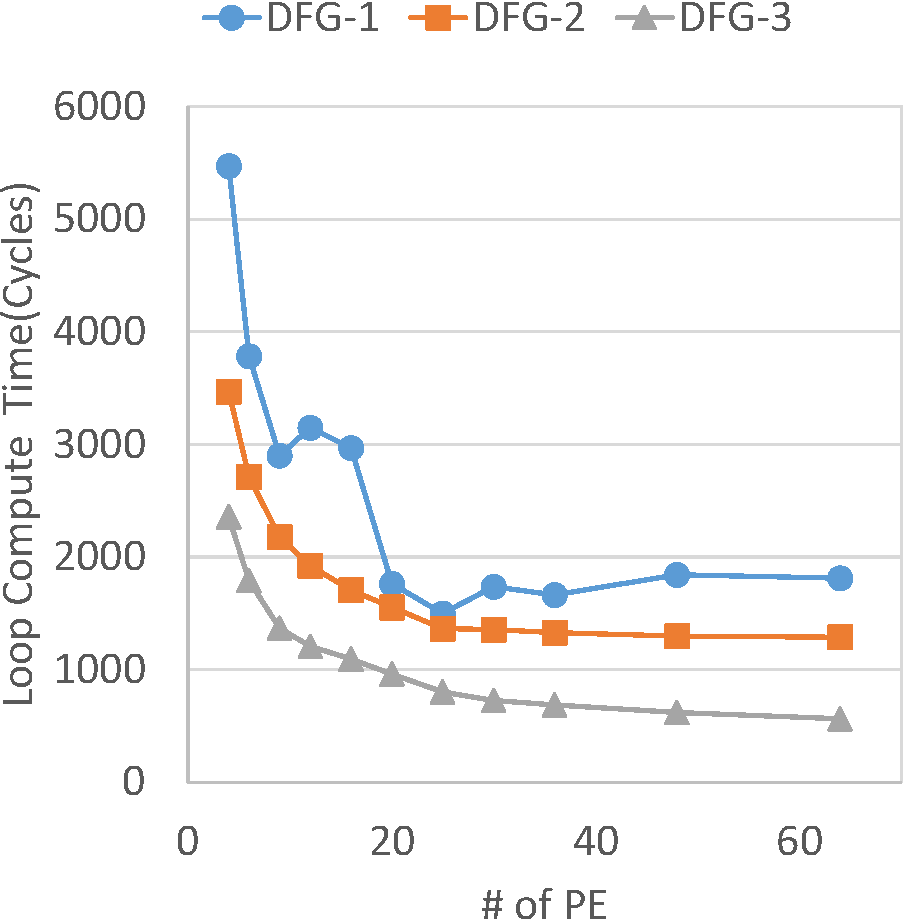
\includegraphics[width=0.235\textwidth]{scgrasize-perf}
    }
    %\hfill
    \subfloat[\label{fig:unrolling-perf}]{%
      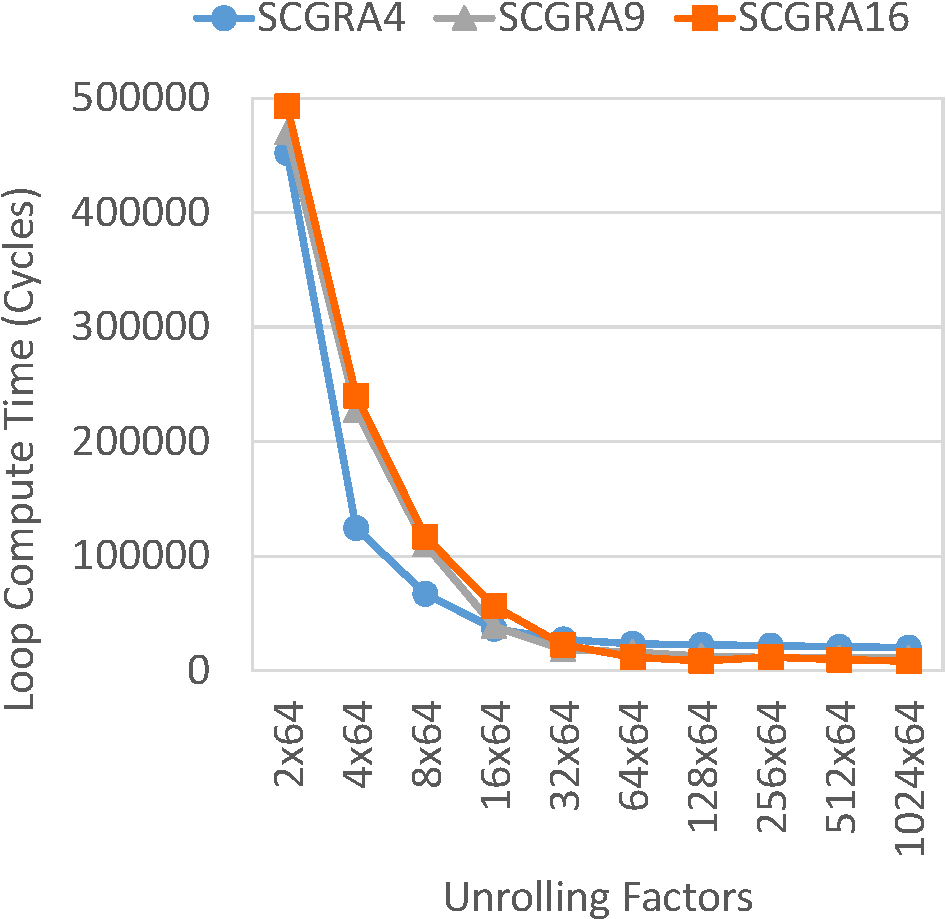
\includegraphics[width=0.22\textwidth]{unrolling-perf}
    }
    \caption{The design parameters typically have monotonic influence on the
        loop computation time and the computation time benefit degrades with 
        the increase of the design parameter. (a) SCGRA Size, (b) Unrolling Factor}
    \label{fig:observation}
  \end{figure}


%\subsection{Sub Design Space Exploration}
%To acquire the FDS, we developed a dedicated sub DSE 
%targeting nested loop computation time. Since the loop computation 
%time merely depends on the SCGRA overlay 
%size and the loop unrolling factor, the sub DSE is much simpler 
%compared to the overall customization problem. In addition, we can 
%further simplify the sub DSE with the observations shown in \figref{fig:observation}.  
%Whenever a configuration fails the sub DSE condition, all the 
%configurations which are larger on one design parameter and remain the same 
%on the rest design parameters can be safely pruned. Thus a branch and 
%bound algorithm as detailed in \algref{alg:revenuealg} is used 
%to efficiently explore the sub design space.
%\begin{algorithm}[h]
%\caption{Sub Design Space Exploration.}
%\label{alg:revenuealg}
%\begin{algorithmic}
%\PROCEDURE{}
%\STATE Initialize $r=2, c=2, \bm{u}=(1,1,...)$, FDS $\Phi=\emptyset$,
%$\bm{C}=(...,r,c,\bm{u},...)$, maximum SCGRA overlay $r_{Max}\times c_{Max}$.
%\WHILE {$r<r_{Max}$} 
%\WHILE {$c<c_{Max}$}
%\WHILE {$\bm{u}$ is not fully unrolled}
%\STATE Generate DFG with $\bm{u}$
%\STATE DFG Scheduling with configuration $\bm{C}$
%\STATE Estimate performance $CompuTime(\bm{C})$
%\STATE Get neighbor $\bm{C'} \in \Phi$ with smaller loop unrolling
%\IF {$\bm{C'}$ exists and $Revenue(\bm{C}, \bm{C'}) \leq \epsilon$}
%\STATE Break
%\ELSE 
%\STATE Add $\bm{C}$ to $\Phi$
%\ENDIF
%\STATE update $\bm{u}$ with larger neighbor unrolling factor
%\ENDWHILE
%\STATE Get neighbor $\bm{C''} \in \Phi$ with smaller column size
%\IF {$\bm{C''}$ exists and $Revenue(\bm{C}, \bm{C''}) \leq \epsilon$}
%\STATE Break
%\ENDIF
%\STATE $c=c+1$
%\ENDWHILE
%\STATE Get neighbor $\bm{C'''} \in \Phi$ with smaller row size
%\IF {$\bm{C'''}$ exists and $Revenue(\bm{C}, \bm{C'''}) \leq \epsilon$}
%\STATE Break
%\ENDIF
%\STATE $r=r+1$
%\ENDWHILE
%\ENDPROCEDURE
%\STATE
%\PROCEDURE {$Revenue(\bm{C}, \bm{C'})$}
%\STATE return $\frac{CompuTime(\bm{C'})-CompuTime(\bm{C})}{CompuTime(\bm{C'})}$ 
%\ENDPROCEDURE
%\end{algorithmic}
%\end{algorithm}
%
%

\section{Experiments and results} \label{sec:result}
The experiments mainly include two parts. In the first part, we 
analyze the implementations of the SCGRA overlay based FPGA accelerators with 
different configurations to demonstrate the regularity of the 
SCGRA overlay based FPGA accelerators. In the second part, we benchmark the 
efficiency and quality of the proposed customization framework.

\subsection{Experiment Setup}
All the run time was obtained from a computer with Intel(R) Core(TM) 
i5-3230M CPU and 8GB RAM. Zedboard which has an ARM processor and 
an FPGA was used as the hybrid computation system. Vivado 2013.3 was 
used for the HLS based design and PlanAhead 14.7 was used for the SCGRA overlay based 
design. 

The overlay implementations on Zedboard typically run at 200MHz and we 
assume the implementation frequency can be scalable to all the 
different overlay configurations. The power consumption used in this work was 
obtained from XPower which is part of the Xilinx design suite.

\subsection{SCGRA Overlay Implementation Analysis}
In order to analyze the overhead and power of the SCGRA overlay 
based FPGA accelerators, we had three groups of accelerators 
(SCGRA1, SCGRA2, SCGRA3) implemented on Zedboard. The configurations 
are detailed in \tabref{tab:config}. Despite of the diverse 
configurations, all the implementations could meet 200MHz 
timing constrain. With this timing constrain, 
hardware overhead and power consumption are analyzed in the 
following sub sections.
\begin{table}[tb]
    \small
    \centering
    \caption{SCGRA Based FPGA Accelerator Configuration \label{tab:config}}{
        \begin{tabular}{c|c|c|c|c|c}
            \hline
            Group & Size & \tabincell{c}{Inst. \\ Rom} & 
            \tabincell{c}{Data \\ Mem} & \tabincell{c}{IBuf \\ /OBuf} & 
            \tabincell{c}{Addr \\Buf} \\ \hline

            SCGRA1 & \tabincell{l}{2x2, 3x2, \\ 3x3, 4x3, \\ 4x4, 5x4} & 
            1kx72 & 256x32 & 2kx32 & 4kx16\\ \hline

            SCGRA2 & \tabincell{l}{2x2, 3x2, \\ 3x3, 4x3, \\4x4} & 
            2kx72 & 256x32 & 2kx32 & 4kx16\\ \hline

            SCGRA3 & \tabincell{l}{2x2, \\ 3x2, \\ 3x3 } &  
            4kx72 & 256x32 & 2kx32 & 4kx16\\ \hline
        \end{tabular}
    }
\end{table}

\subsubsection{Hardware Overhead}
\figref{fig:SCGRA-Overhead} shows the relation between 
the four types of hardware resource overhead and SCGRA 
overlay size. It can be found that FF, LUT and DSP overhead 
do not change much with the memory configurations and they 
present good linearity to the overlay size, thus they can be 
estimated with linear models. BRAM overhead depends 
on both the overlay size and the memory configurations, 
and single variable linear model will not work for the estimation.
Fortunately, it can be calculated precisely with the memory 
configurations. 

\begin{figure}[tb]
    \subfloat[\label{fig:FF-Overhead}]{%
      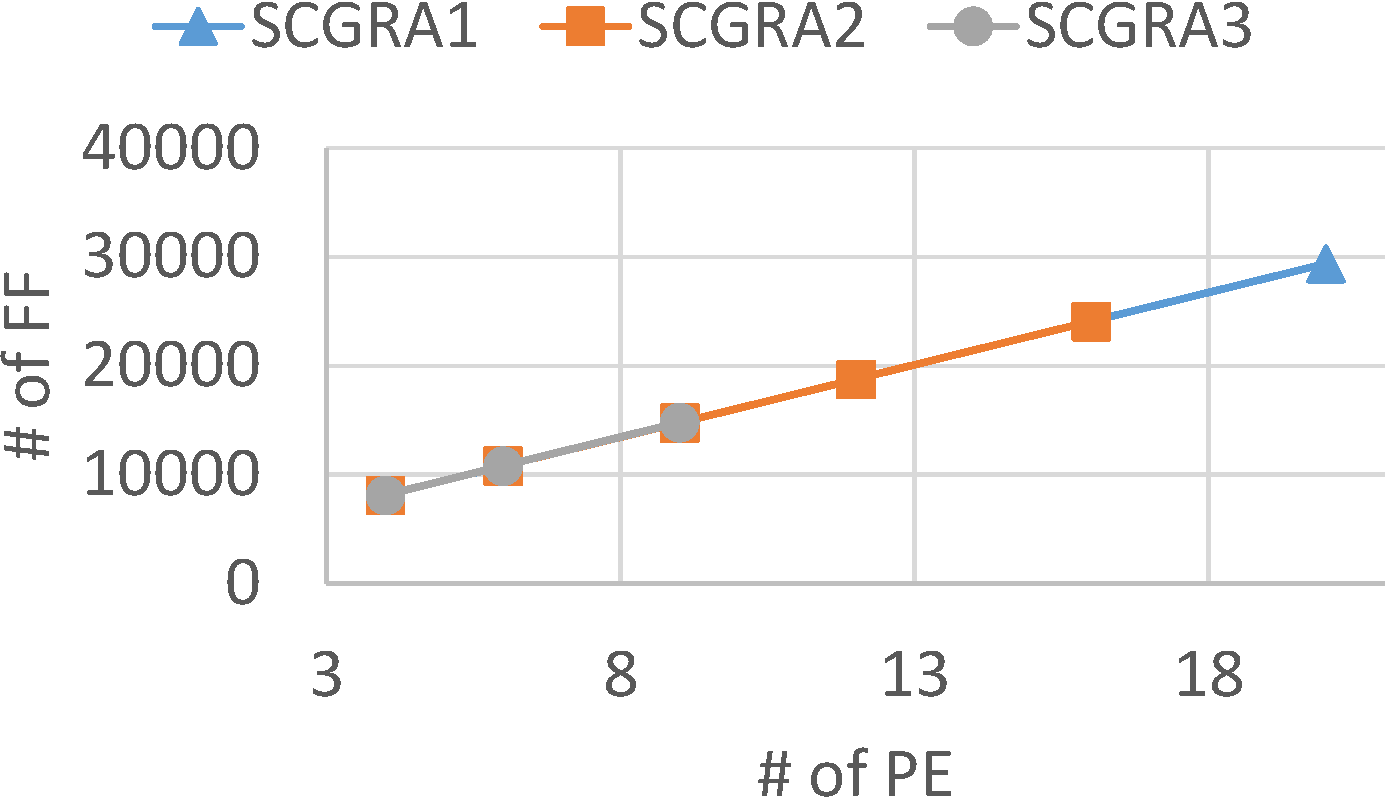
\includegraphics[width=0.22\textwidth]{FF-Overhead}
    }
    \subfloat[\label{fig:LUT-Overhead}]{%
      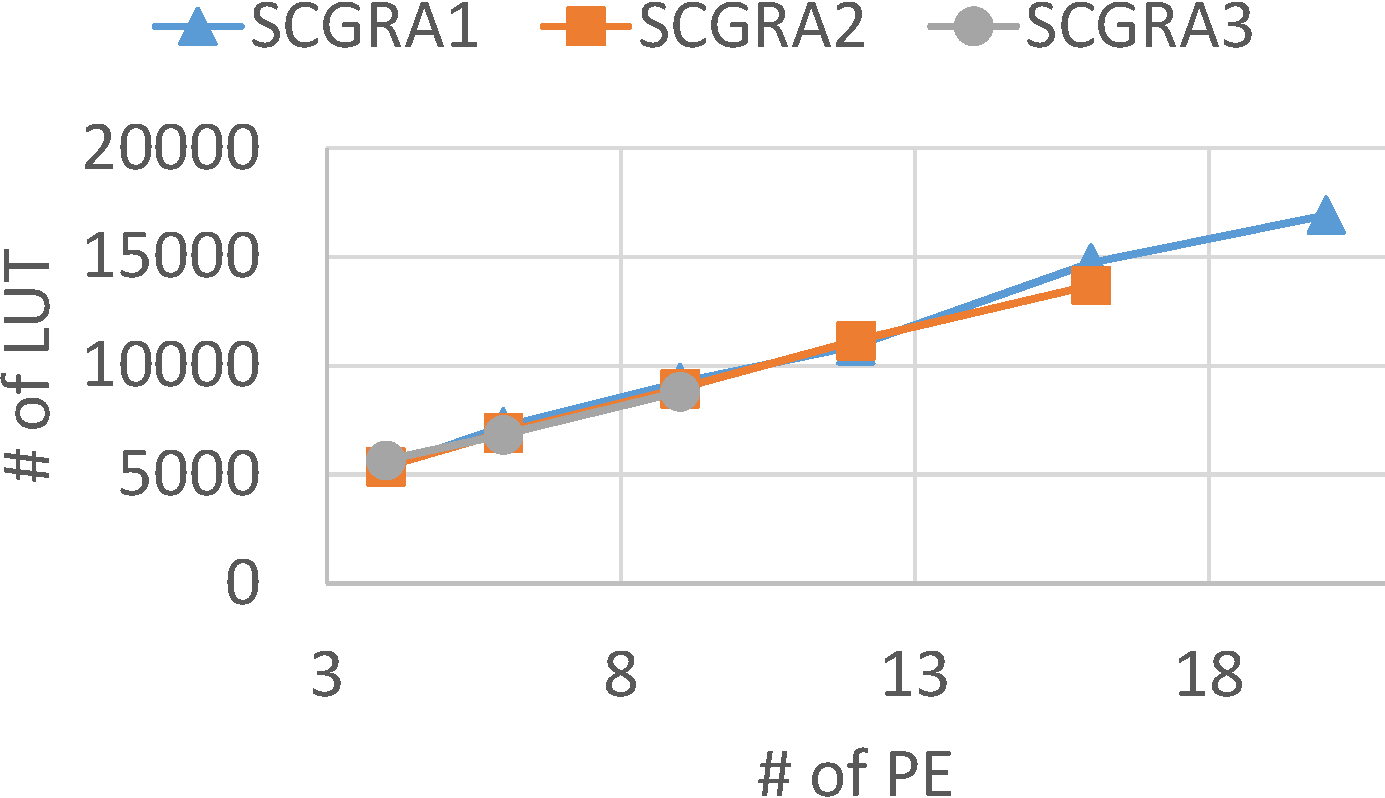
\includegraphics[width=0.22\textwidth]{LUT-Overhead}
    }
    \hfill
    \subfloat[\label{fig:DSP-Overhead}]{%
      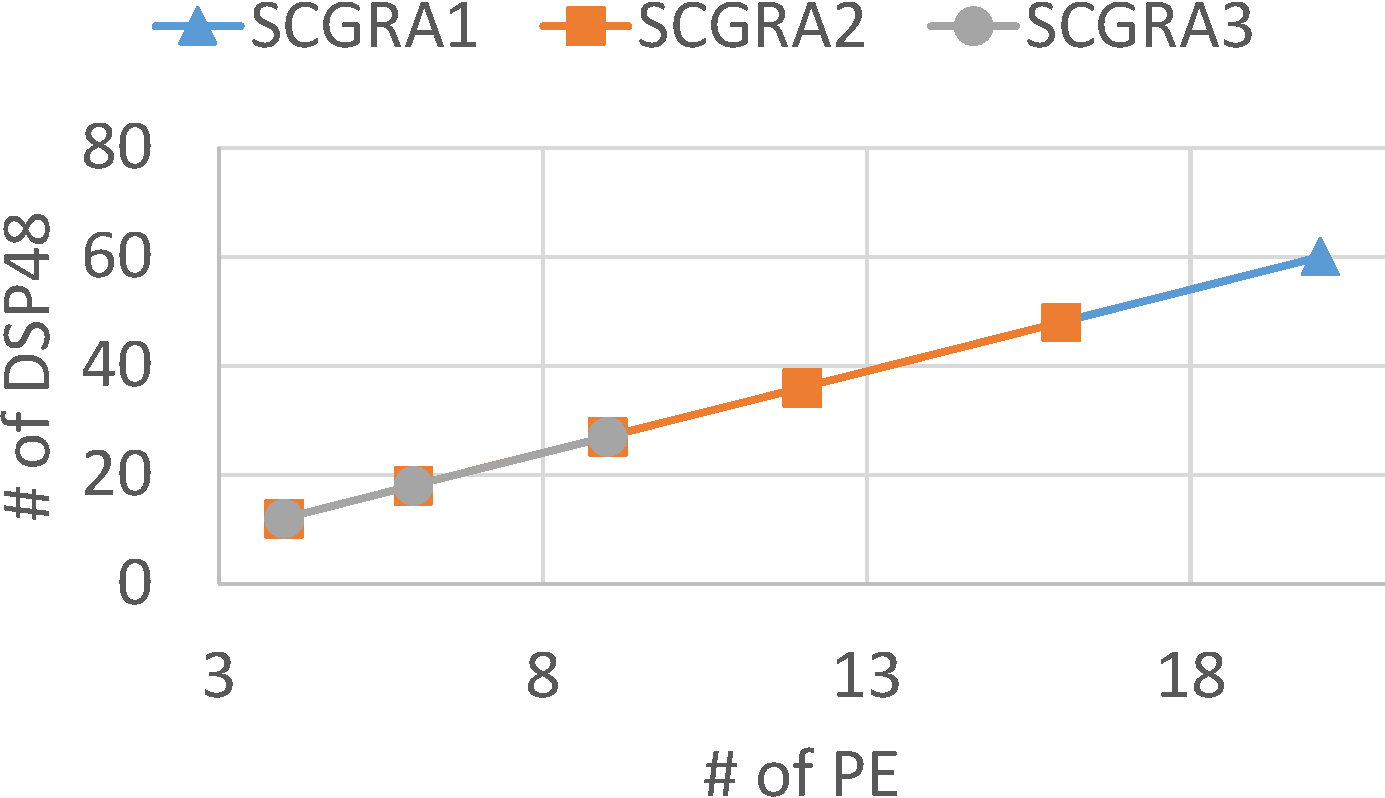
\includegraphics[width=0.22\textwidth]{DSP-Overhead}
    }
    \subfloat[\label{fig:BRAM-Overhead}]{%
      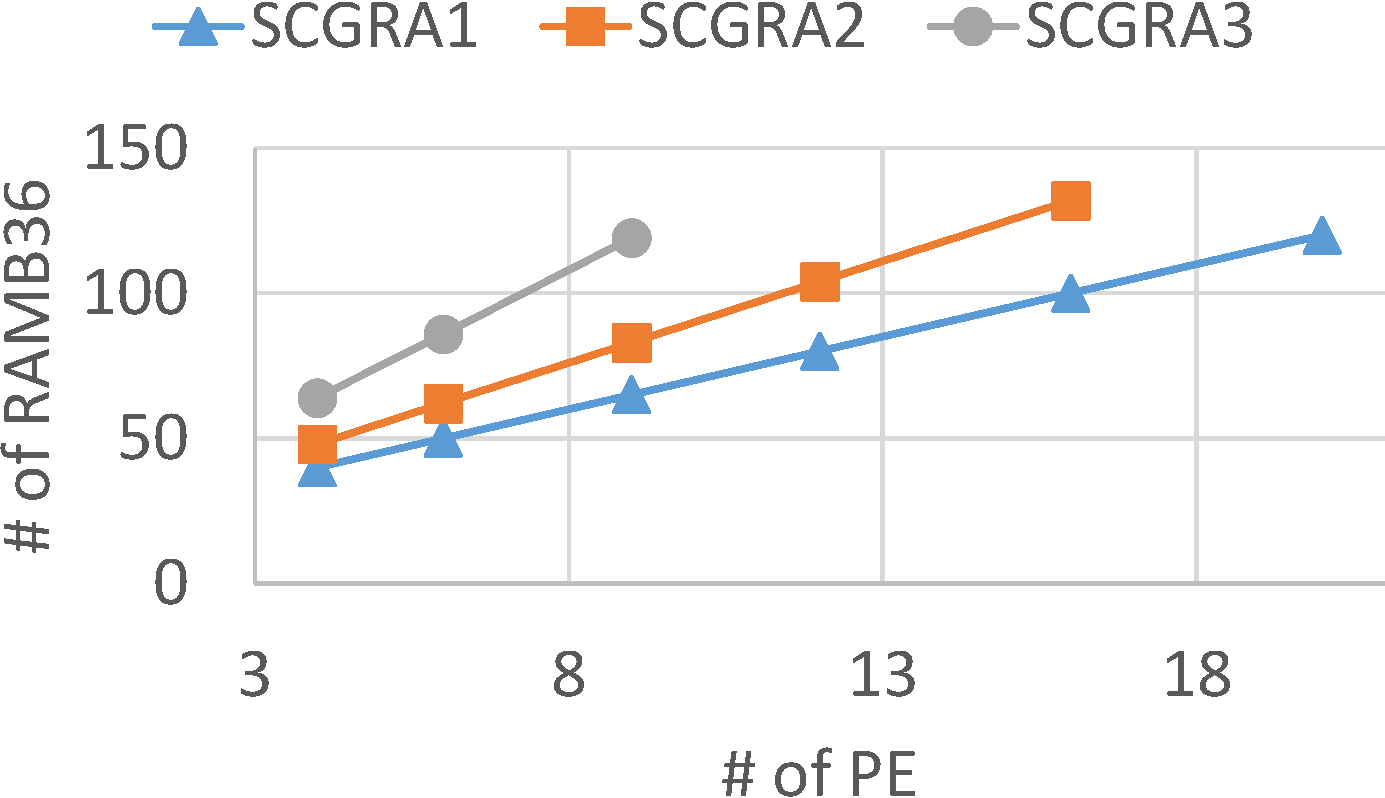
\includegraphics[width=0.22\textwidth]{BRAM-Overhead}
    }
    \caption{Relation between the accelerator overhead and overlay size, 
    (a) FF overhead, (b) LUT overhead, (c)DSP overhead, (d)BRAM overhead}
    \label{fig:SCGRA-Overhead}
\end{figure}


\subsubsection{Power Consumption}
According to the power decomposition in Xpower, the power consumption 
of an FPGA design includes signal power, clock power, BRAM power and so on. 
To simplify the power model of the SCGRA overlay based FPGA accelerator, 
we divide the power consumption into BRAM power and base system 
power which essentially includes the power consumption of the rest part of the system. 
As shown in \figref{fig:SCGRA-Power}, the base system power exhibits good linearity 
over the SCGRA overlay size while the BRAM power is near linear to 
the BRAM overhead. Therefore, both of them can be easily estimated with linear models. 

\begin{figure}[tb]
    \subfloat[\label{fig:Base-Power}]{%
      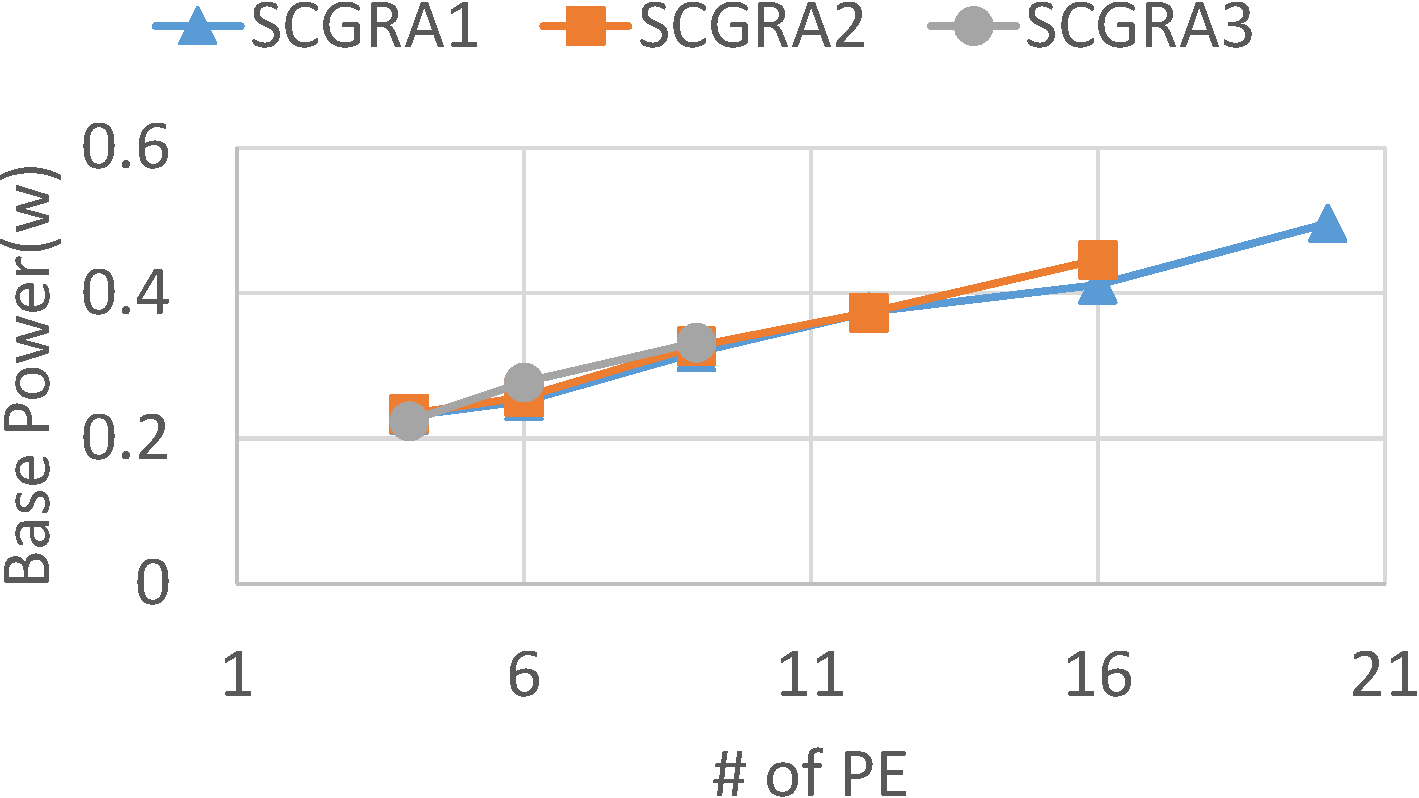
\includegraphics[width=0.22\textwidth]{Base-Power}
    }
    \subfloat[\label{fig:BRAM-Power}]{%
      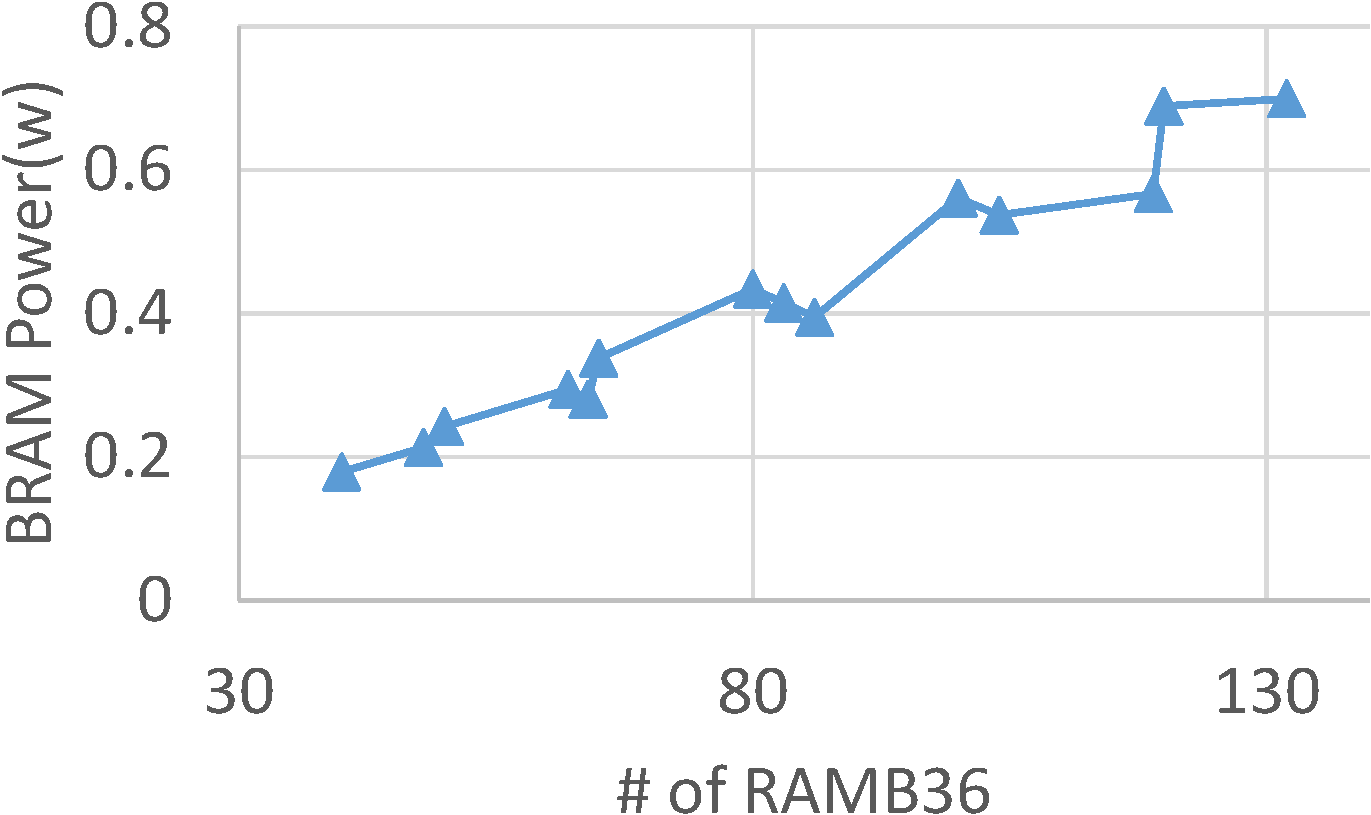
\includegraphics[width=0.22\textwidth]{BRAM-Power}
    }
    \caption{Power consumption of the SCGRA overlay based FPGA accelerator, 
    (a) Base system power including DSP power, clock power, etc., (b) BRAM power}
    \label{fig:SCGRA-Power}
\end{figure}

\subsection{Proposed Design Framework Evaluation}
In this work, we take four applications including Matrix Multiplication (MM), 
FIR, Kmean(KM) and Sobel Edge Detector (SE) as our benchmark. The 
configurations of the benchmark are detailed in \tabref{tab:benchmark-config}. 
In order to evaluate the efficiency and quality of the proposed design 
framework, we have the benchmark implemented using both the proposed 
two-step customization (TS) method and an exhaustive search (ES) 
method. Then we compared the Pareto-optimal curves acquired 
using both methods. In addition, we also have the benchmark 
implemented using Vivado HLS with moderate manual optimization 
and compare the implementations with our customized implementations. 

\begin{table}[tb]
    \small
    \centering
    \caption{Benchmark Configurations \label{tab:benchmark-config}}{
        \begin{tabular}{l|l|l}
            \hline
            Benchmark & Parameters & Loop Structure \\ \hline
            MM & Matrix Size(128) & $128 \times 128 \times 128$ \\ \hline
            FIR & \tabincell{l}{\# of Input (1024) \\ \# of Taps+1 (64)} & $1024 \times 64$ \\ \hline
            SE & \tabincell{l}{ \# of Vertical Pixels (128) \\ \# of Horizontal Pixels (8)} & $128 \times 8 \times 3 \times 3$ \\ \hline 
            KM & \tabincell{l}{\# of Nodes(1024) \\ \# of Centroids(4) \\ \# of Dimensions(2)} & $1024 \times 4 \times 2$ \\ \hline  
        \end{tabular}
    }
\end{table}

\subsubsection{Customization Methods Comparison}
\figref{fig:DSE-Time} shows the DSE time of both the TS DSE and ES DSE. 
The proposed TS DSE is around 100x faster than the ES DSE on 
average. In particular, it can be found that ES DSE can be 
extremely slow on MM which has three levels of loop with relatively large 
loop count and thus larger design space. Though TS DSE also needs 
longer time to complete the DSE of MM, it can skip most 
of the unfeasible configurations and the runtime is 
less sensitive to the size of the design space. 

\begin{figure}[tb]
    \centering
    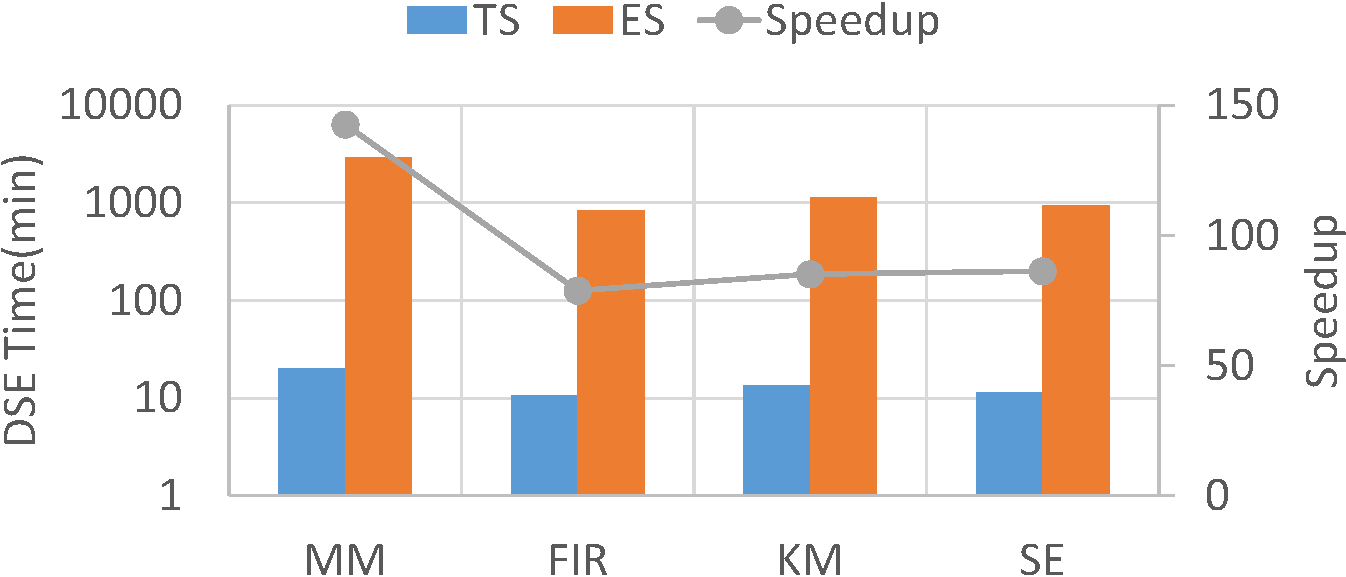
\includegraphics[width=0.35\textwidth]{DSE-Time}
    \caption{DSE time of the benchmark using both TS and ES}
    \label{fig:DSE-Time}
\end{figure}

%\begin{table}[tb]
%    \small
%    \centering
%    \caption{Time Cost for RA DSE and ES DSE\label{tab:dsetime}}{
%        \begin{tabular}{l|l|l|l|l}
%            \hline
%            Benchmark & MM & FIR & KM & SE \\ \hline
%            RA DSE (min) & 20.2 & 10.6 & 13.4 & 11.4\\ \hline
%            ES DSE (min) & 2880.6 & 835.2 & 1140.5 & 946.2\\ \hline
%            Speedup & 142.6 & 78.8 & 85.1 & 86.2 \\ \hline
%        \end{tabular}
%    }
%\end{table}

In order to demonstrate the quality of proposed framework, we presented the 
Pareto-optimal curves acquired from both DSE methods as shown in \figref{fig:DSE}. 
It is clear that the Pareto-optimal curves obtained via the two DSE methods are quite 
close. Since TS DSE may prune the design options that involve a larger 
overlay size and better performance according to the sub DSE metric, 
the Pareto-optimal curves may deviate slightly at the higher performance area. 
Fortunately, this can be improved by lowering user defined metric $\epsilon$ 
while affording longer DSE time. When we customize the design for minimum energy 
consumption, TS DSE can achieve the optimal design in all the benchmarks. 

\begin{figure}[tb]
	\subfloat[MM]{%
		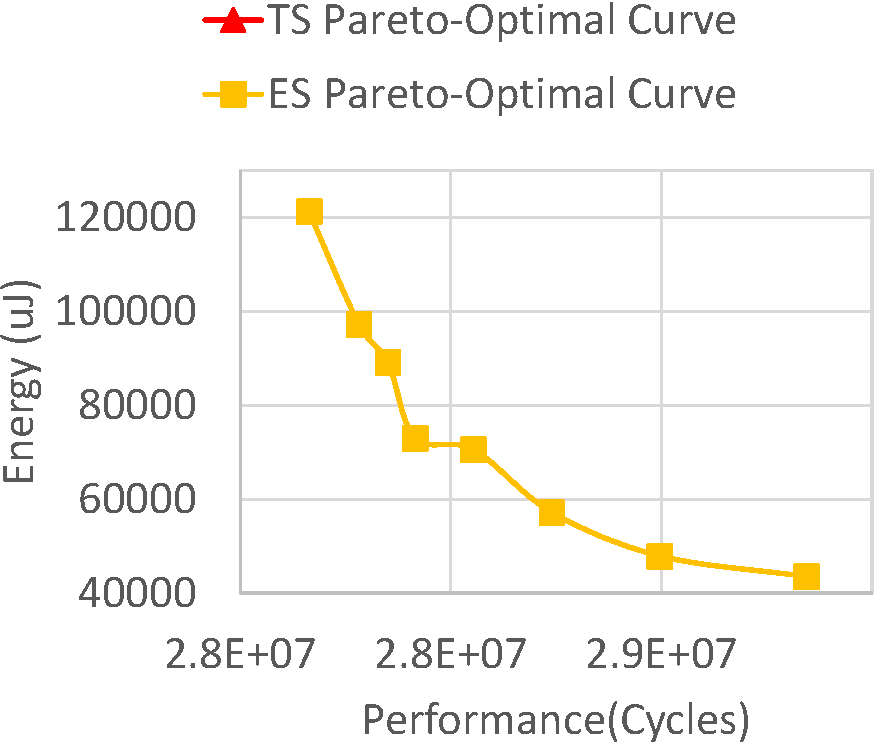
\includegraphics[width=0.22\textwidth]{mm-energy-performance}
	}
	\subfloat[FIR]{%
		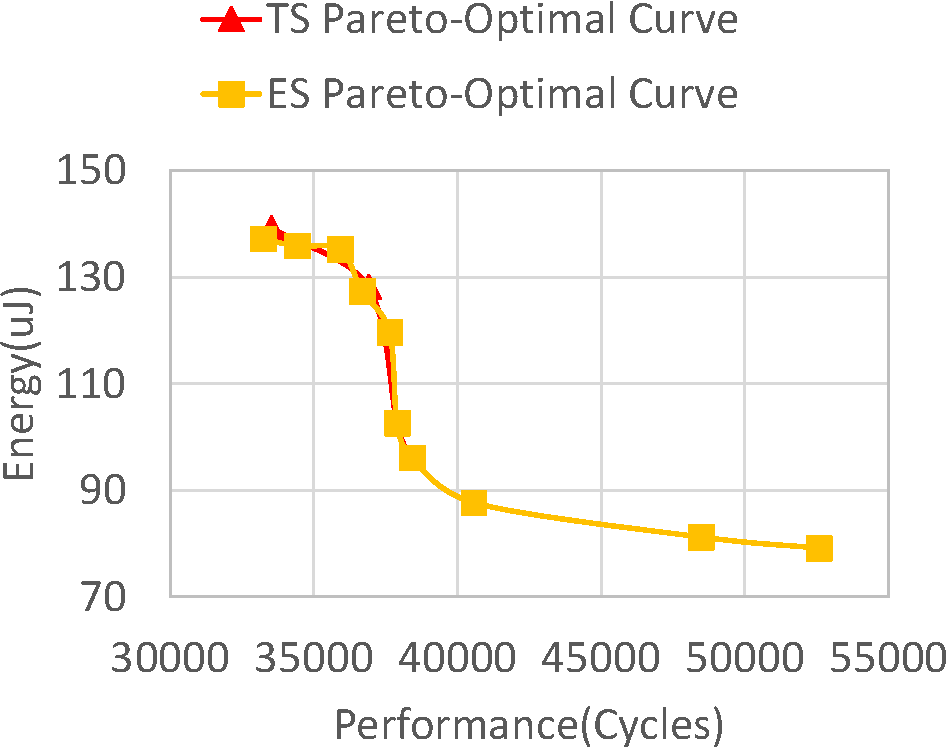
\includegraphics[width=0.22\textwidth]{fir-energy-performance}
	}
    \hfill
	\subfloat[SE]{%
		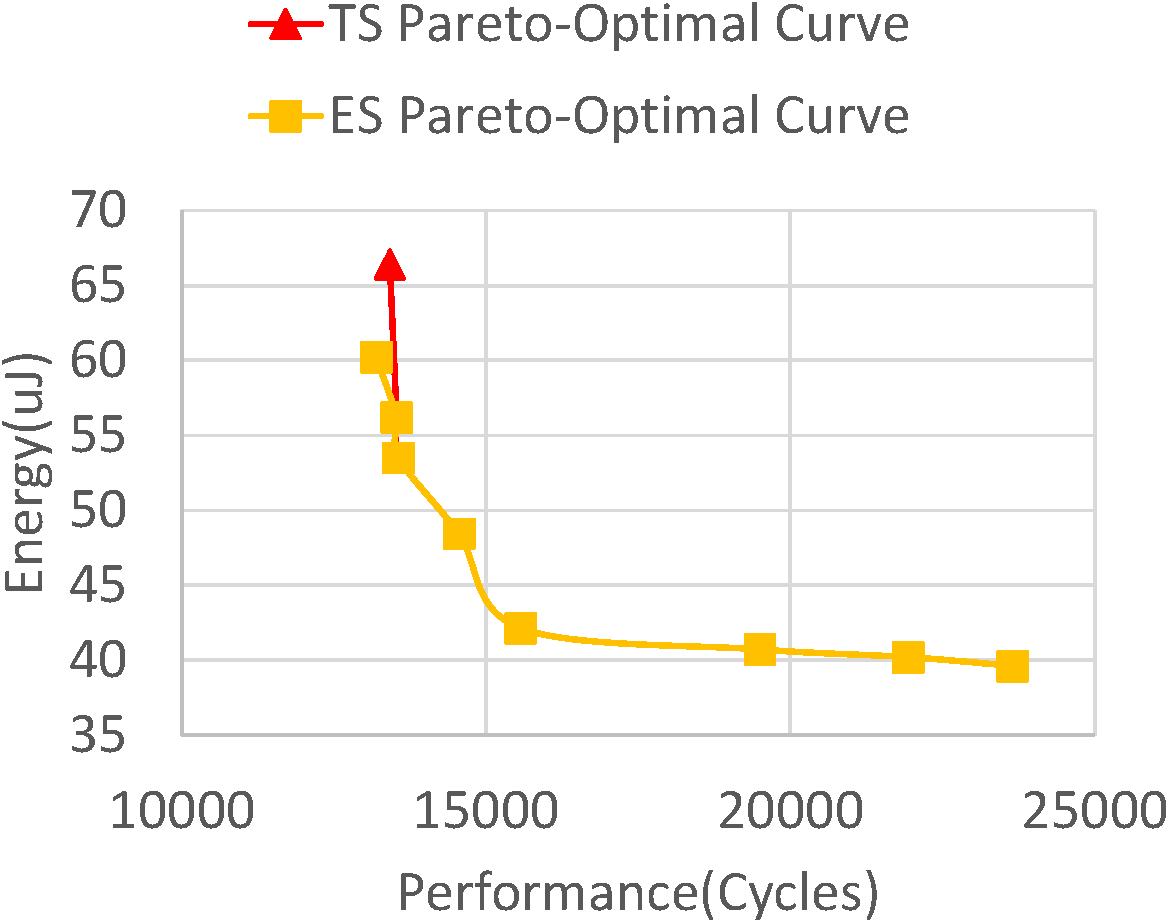
\includegraphics[width=0.22\textwidth]{se-energy-performance}
	}
	\subfloat[KM]{%
		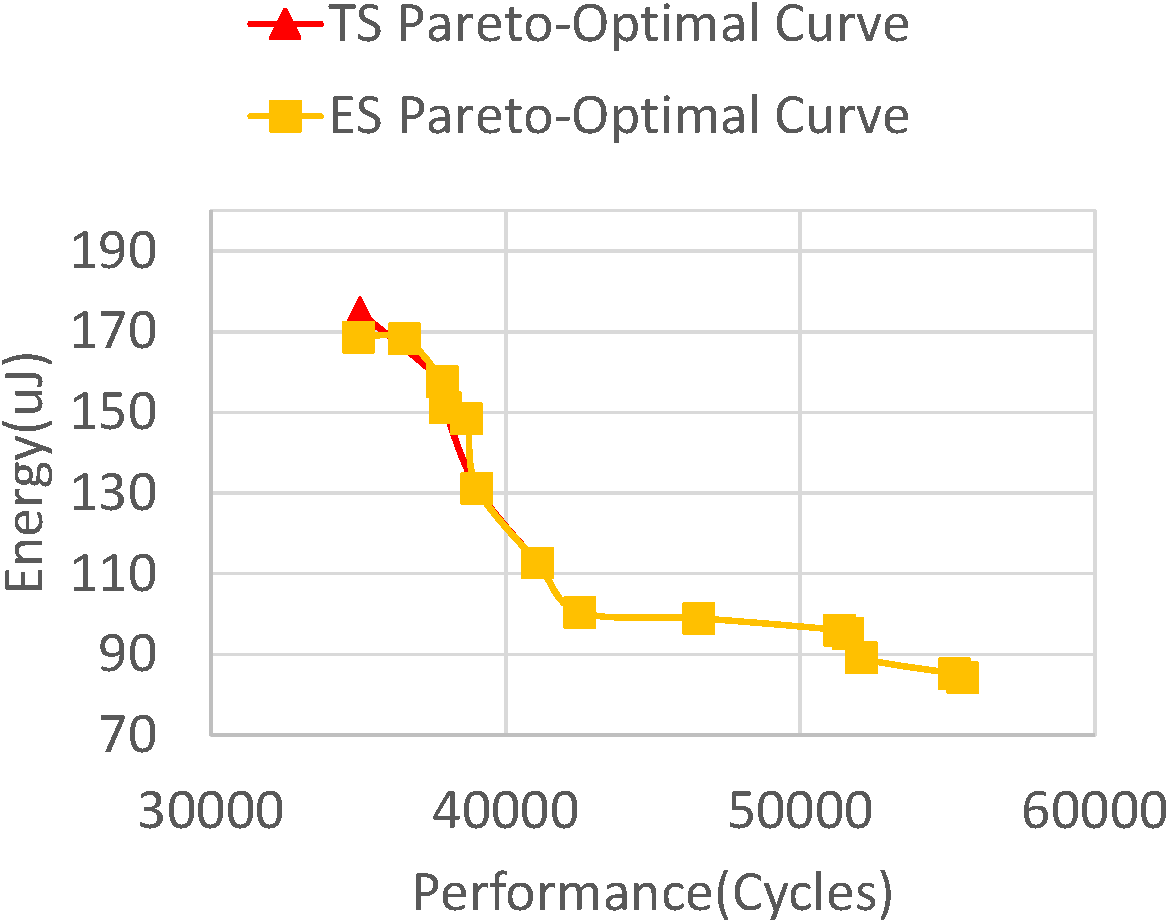
\includegraphics[width=0.22\textwidth]{km-energy-performance}
	}
    \caption{Performance-Energy Pareto-optimal curve}
	\label{fig:DSE}
\end{figure}

\subsubsection{Design Tools Comparison}
The proposed design framework will not be as useful if the performance of the 
generated system is not at least on par with similar systems created with 
conventional high-level synthesis tools. For that, we further implemented the 
benchmarks using Vivado HLS with moderate effort. The loops in the benchmark will 
be unrolled as much as possible and the input/output buffers are set as large 
as possible. Then the accelerators generated using both tools are compared. 
Since similar comparison has already been done in previous work \cite{scgra-orig}, 
we just brief the performance comparison for a quick reference.

\begin{figure}[tb]
	\subfloat[MM]{%
		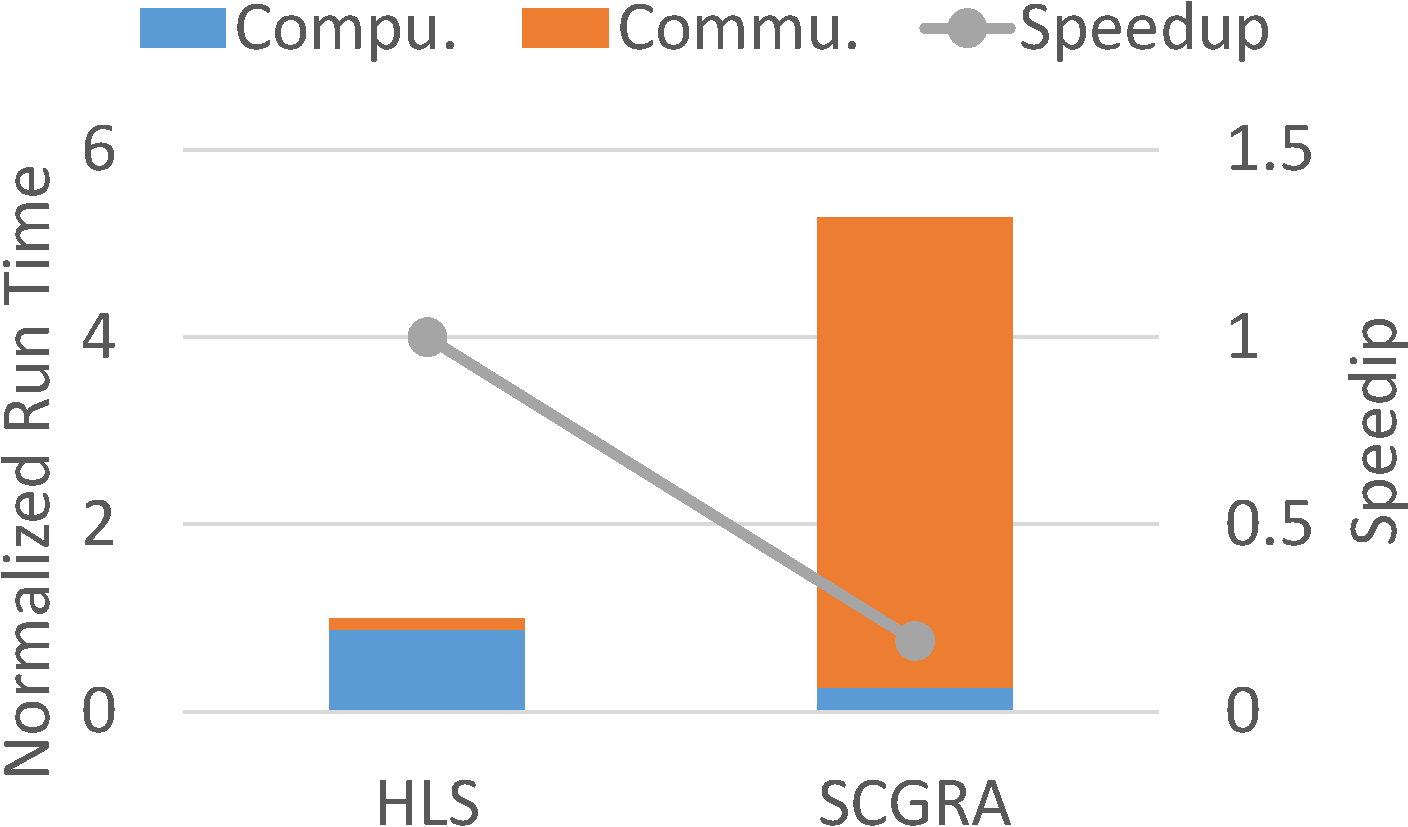
\includegraphics[width=0.22\textwidth]{mm-hls-cp}
	}
	\subfloat[FIR]{%
		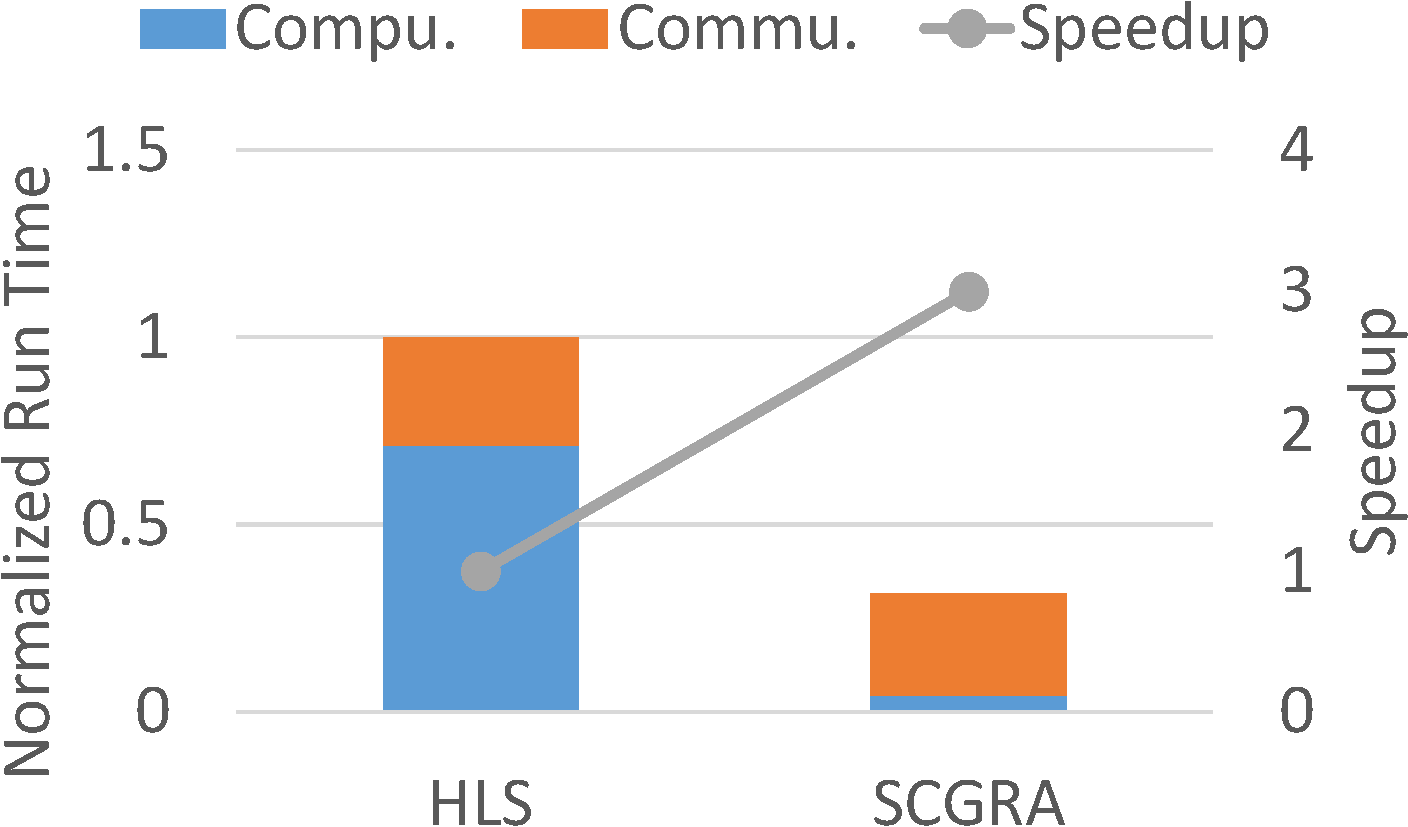
\includegraphics[width=0.22\textwidth]{fir-hls-cp}
	}
    \hfill
	\subfloat[SE]{%
		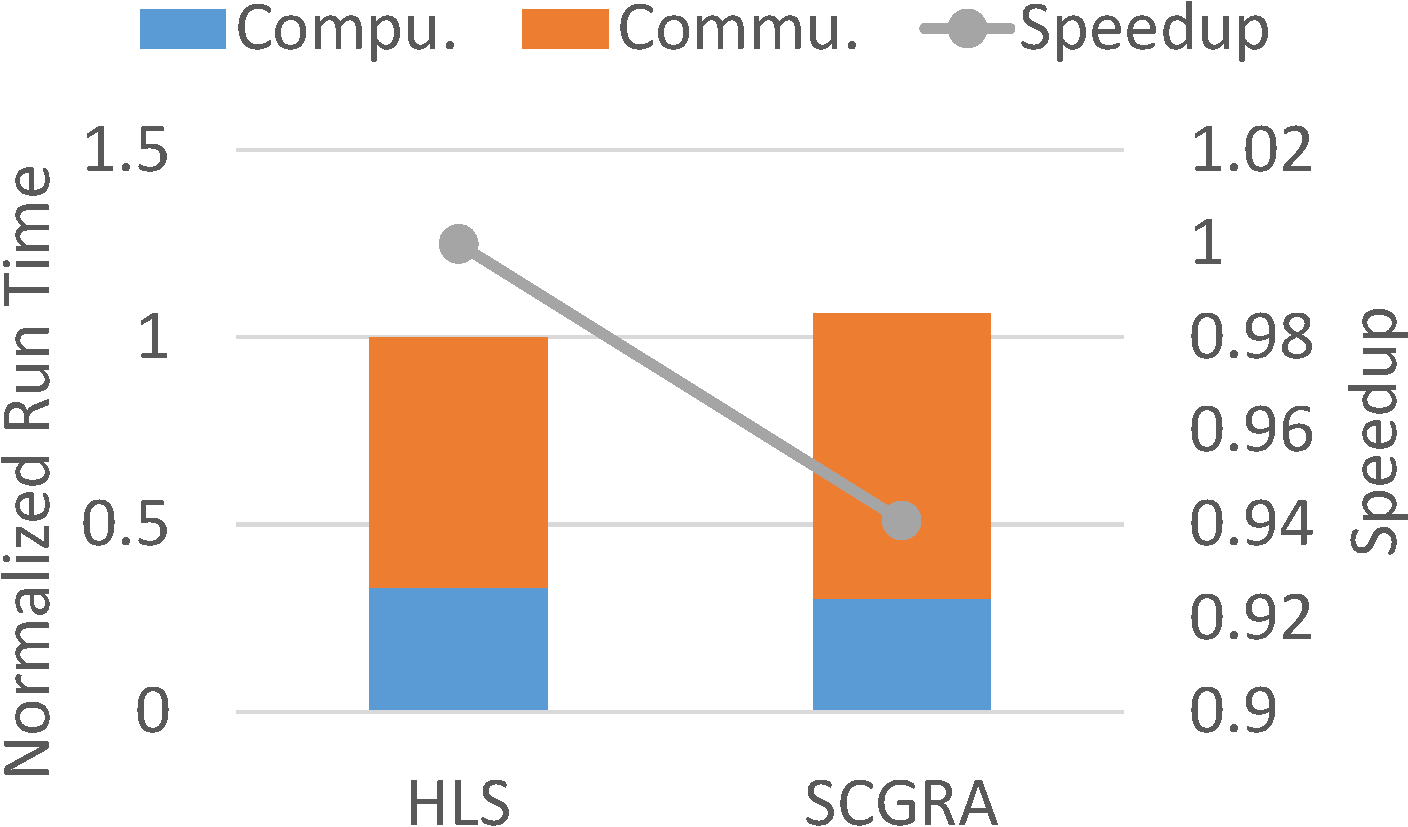
\includegraphics[width=0.22\textwidth]{se-hls-cp}
	}
	\subfloat[KM]{%
		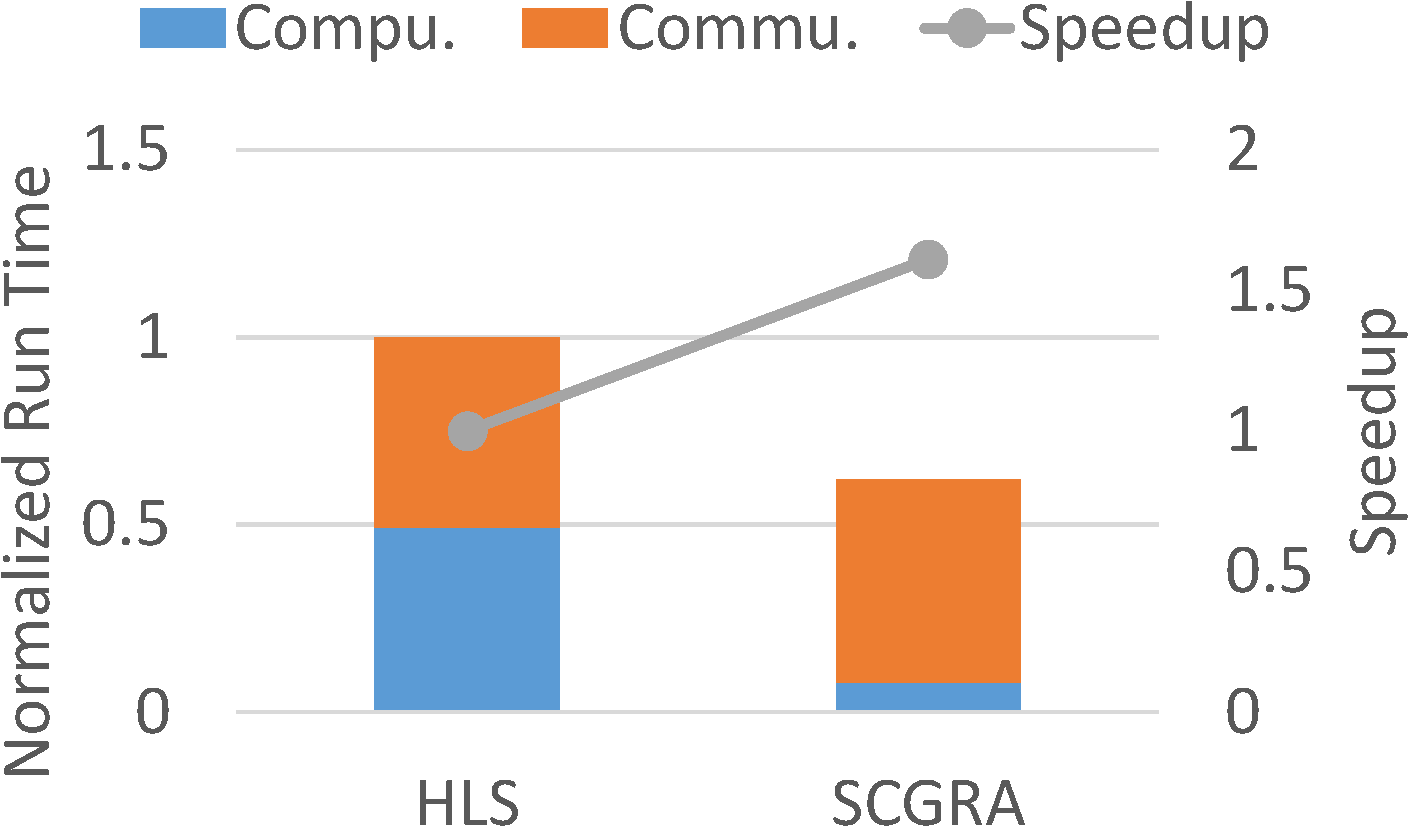
\includegraphics[width=0.22\textwidth]{km-hls-cp}
	}
    \caption{Performance comparison between the implementations 
        using HLS and the proposed automatic customization framework.
    All the run time is normalized to that of the HLS based implementations.}
	\label{fig:hls-cp}
\end{figure}


\figref{fig:hls-cp} shows the performance of the implementations using 
both design tools. The proposed customization framework utilizes 
SCGRA overlay as the backbone and it can't afford large 
BRAM for input/output buffers. As a result, the communication time is larger 
especially when there is a lot of data reuse between consecutive data transmission.
For instance, HLS based design can afford a 32k-word input buffer storing all 
the input data. However, the SCGRA overlay based design can only 
provide a 4k-word input buffer and it needs to transmit the same data 
multiple times to complete the matrix multiplication. Direct HLS can't support large 
loop unrolling due to the DSP resource constrain. SCGRA overlay based accelerator 
has a lot of distributed intermediate buffers and can accommodate larger loop unrolling.
Therefore, the accelerators generated using the proposed framework provides competitive 
pure computation time and overall performance especially for compute intensive loops.



\section{Conclusion} \label{sec:Conclusion}
In this work, we propose to replace the forward computing on GPPs with accelerator 
computing during training and have both the computing 
errors and the application data learned in the neural network models. 
In addition, we opt to protect critical neural layers to reduce the negative 
influence of computing errors.  
With the proposed resilient neural network training, 
the prediction accuracy of the retrained neural network models improves significantly 
when computing errors appear. 


%\appendix
%\section{Acknowledgement}

%\begin{acks}
%  The authors would like to thank Sam Ho for providing the suggestions on
%  HLS design debugging and optimization as well as the SDAccel usage. 

%\end{acks}


\section*{Acknowledgment}
This work was supported in part by the Research Grants Council of Hong Kong project ECS 720012E and
the Croucher Innovation Award 2013. 


\bibliographystyle{IEEEtran}
\bibliography{refs,ieeebstctl}

%\balancecolumns
\end{document}

